\documentclass[lettersize,journal]{IEEEtran}
\usepackage{bm}
\usepackage{verbatim}
\usepackage{calc}
\usepackage{algorithm2e}
\usepackage{array}
\usepackage{booktabs}
\usepackage{colortbl}
\usepackage{supertabular}
\usepackage{amsmath,amsfonts}
\usepackage{tikz}
\usepackage{subfig}
\hyphenation{op-tical net-works semi-conduc-tor IEEE-Xplore}
\def\BibTeX{{\rm B\kern-.05em{\sc i\kern-.025em b}\kern-.08em
    T\kern-.1667em\lower.7ex\hbox{E}\kern-.125emX}}
\usepackage{balance}
\usepackage[backend=bibtex, style=numeric, sorting=none]{biblatex}
\bibliography{references}

\begin{document}
\title{A Light Weight Approach to Minimize Charging Cost for Electric Bus Fleets}
\author{Daniel Mortensen, Jacob Gunther\thanks{}}

\markboth{Transactions on Intelligent Transportation Systems}%
{}

\maketitle 
\begin{abstract}
\textcolor{red}{Insert abstract here}
\end{abstract}

\begin{IEEEkeywords}
\textcolor{red}{Insert keywords here}
\end{IEEEkeywords}

\input{2_introduction.tex}
\input{3_formulation.tex}
\input{4_battery.tex}
\section{Charger Management}
\par Limited numbers of chargers is another limitation that many transit authorities face.  Let the number of chargers be denoted $n_{\text{charger}}$. We desire to maintain the average cumulative power for each time step at a level that is serviceable given $n_{\text{charger}}$. We define a slack variable $p_c(j)$ which represents the total average power consumed by all buses at time $j$.  The variable $p_c(j)$ is computed as the sum of average bus powers so that
\begin{equation*}
	p_c(j) = \sum_ib_{p(i,j)}
\end{equation*}
or also as 
\begin{equation}
p_c(j) - \sum_ib_{p(i,j)}  = 0\ \forall j.
\end{equation}
\par From a practical standpoint, we must also avoid multiple charging sessions in one visit to the station, or charger thrashing. We to this by minimising the difference in the average power values throughout the day.  When a bus uses the charger for longer periods of time, the average power remains the same for multiple time periods.  If a bus reconnects/disconnects multiple times, there will be larger difference in the power use from one time period to another. This can be expressed as
\begin{equation}
	J_{\text{thrash}} = \sum_{i,j > 1} \lvert b_{p(i,j)} - b_{p(i,j-1)}\rvert.
\end{equation}
To minimize $J_{\text{thrash}}$, we define a slack variable $g_{i,j}$ so that 
\begin{equation*}
g_{i,j} = \lvert b_{p(i,j)} - b_{p(i,j-1)} \rvert.
\end{equation*}
which can be enforced by the linear constraints 
\begin{equation*}\begin{aligned}
	-g_{i,j} &\le b_{p(i,j)} - b_{p(i,j-1)} \\
	g_{i,j} &\ge b_{p(i,j)} - b_{p(i,j-1)}.
\end{aligned}\end{equation*}
Suppose $b_{p(i,j)} - b_{p(i,j-1)} = -5$, then we have 
\begin{equation*}
	-g \le -5 \le g
\end{equation*}
which minimizes $g$ when $g = 5$. A similar expression is minimized when $g$ is positive. The expression for $g_{i,j}$ can alternatively be expressed in standard form as
\begin{equation}\begin{aligned}
-g_{i,j} - b_{p(i,j)} + b_{p(i,j-1)} \le 0 \\
-g_{i,j} + b_{p(i,j)} - b_{p(i,j-1)} \le 0.
\end{aligned}\end{equation}


\input{6_objective.tex}
% imports
\begin{figure*}
\centering
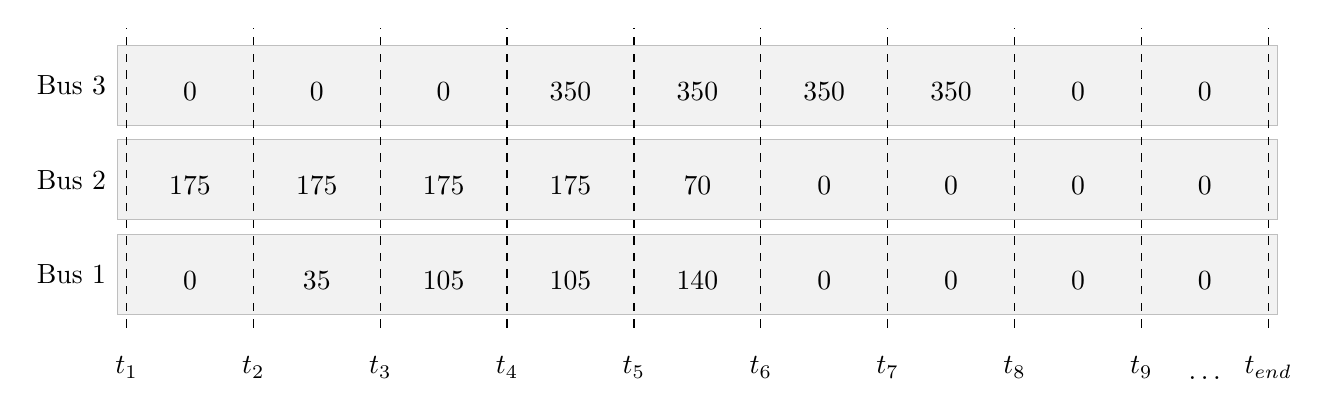
\begin{tikzpicture}
	\node[rectangle, draw=gray!50, fill=gray!10, minimum width=5.8in, minimum height=0.4in](bus1Box) at (7.75,0.8){};
	\node(bus1BoxLabel) at (-0.2, 0.8){Bus 1}; 
	
	\node[rectangle, draw=gray!50, fill=gray!10, minimum width=5.8in, minimum height=0.4in](bus2Box) at (7.75,2){};
	\node(bus1BoxLabel) at (-0.2, 2.0){Bus 2};
	
	\node[rectangle, draw=gray!50, fill=gray!10, minimum width=5.8in, minimum height=0.4in](bus3Box) at (7.75,3.2){};
	\node(bus1BoxLabel) at (-0.2, 3.2){Bus 3};
	
	\foreach \curLab/\preLab[count=\c, evaluate=\c as \pos using {0.5 + (\c - 1)*14.5/9}] in {t_1/t_1, t_2/t_1, t_3/t_2, t_4/t_3, t_5/t_4, t_6/t_7, t_7/t_6, t_8/t_7, t_9/t_8, t_{end}/t_9}
	{
		\node[label=below:$\curLab$](b\c) at (\pos, 0){};
		\node(t) at (\pos, 3.8){};
		\draw[dashed, line width=0.5pt] (b\c.north) -- (t.north); 
		\ifnum\c>1 
			\node(b1Curr) at (\pos, 0.8 - 0.2){};
			\node(b2Curr) at (\pos, 2.0 - 0.2){};
			\node(b3Curr) at (\pos, 3.2 - 0.2){};
			\path(b1Prev.east) -- node(node1\c)[midway, above]{}(b1Curr.west);
			\path(b2Prev.east) -- node(node2\c)[midway, above]{}(b2Curr.west);
			\path(b3Prev.east) -- node(node3\c)[midway, above]{}(b3Curr.west);	
		\fi
			\node(b1Prev) at (\pos, 0.8 - 0.2){};
			\node(b2Prev) at (\pos, 2.0 - 0.2){};
			\node(b3Prev) at (\pos, 3.2 - 0.2){};	
	}
	\path (b9.south) -- node[midway, below=0.1in]{$\hdots$}(b10.south);
	\node at (node12.center){0};
	\node at (node13.center){35};
	\node at (node14.center){105};
	\node at (node15.center){105};
	\node at (node16.center){140};
	\node at (node17.center){0};
	\node at (node18.center){0};
	\node at (node19.center){0};
	\node at (node110.center){0};
	\node at (node22.center){175};
	\node at (node23.center){175};
	\node at (node24.center){175};
	\node at (node25.center){175};
	\node at (node26.center){70};
	\node at (node27.center){0};
	\node at (node28.center){0};
	\node at (node29.center){0};
	\node at (node210.center){0};
	\node at (node32.center){0};
	\node at (node33.center){0};
	\node at (node34.center){0};
	\node at (node35.center){350};
	\node at (node36.center){350};
	\node at (node37.center){350};
	\node at (node38.center){350};
	\node at (node39.center){0};
	\node at (node310.center){0};

\end{tikzpicture}
\caption{An example solution to a 3-bus, 2-charger scenario from the first QP}
\label{fig:solutionExample}
\end{figure*}

\begin{figure*}
\centering
\scalebox{0.8}{
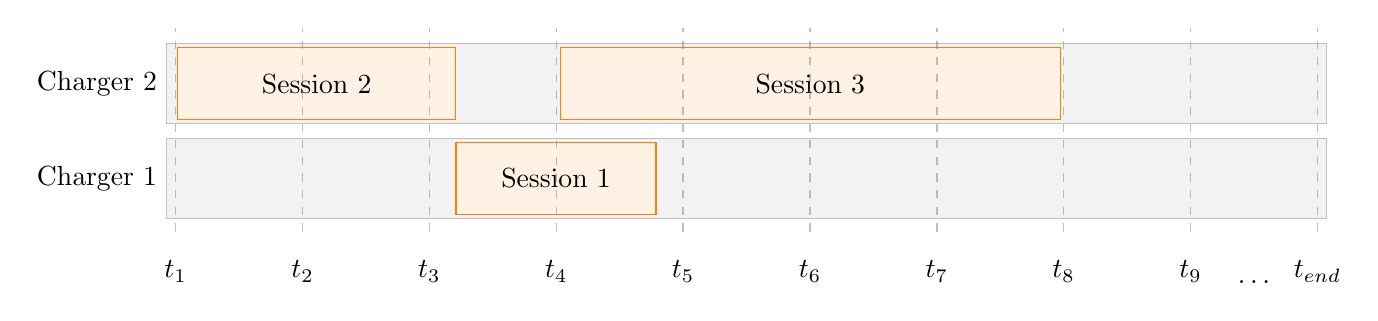
\begin{tikzpicture}
	\node[rectangle, draw=gray!50, fill=gray!10, minimum width=5.8in, minimum height=0.4in](bus1Box) at (7.75,0.8){};
	\node(bus1BoxLabel) at (-0.5, 0.8){Charger 1}; 

	\node[rectangle, draw=gray!50, fill=gray!10, minimum width=5.8in, minimum height=0.4in](bus2Box) at (7.75,2){};
	\node(bus1BoxLabel) at (-0.5, 2.0){Charger 2};
	\node[rectangle, draw=orange!100, fill=orange!10, minimum width=1.3915in, minimum height=0.36in](charge111) at (2.29, 2){Session 2}; 
	\node[rectangle, draw=orange!100, fill=orange!10, minimum width=1in, minimum height=0.36in](charge111) at (5.33, 0.8){Session 1};
	\node[rectangle, draw=orange!100, fill=orange!10, minimum width=2.50in, minimum height=0.36in](charge111) at (8.56, 2){Session 3};


	\foreach \curLab/\preLab[count=\c, evaluate=\c as \pos using {0.5 + (\c - 1)*14.5/9}] in {t_1/t_1, t_2/t_1, t_3/t_2, t_4/t_3, t_5/t_4, t_6/t_7, t_7/t_6, t_8/t_7, t_9/t_8, t_{end}/t_9}
		{
			\node[label=below:$\curLab$](b\c) at (\pos, 0){};
			\node(t) at (\pos, 2.58){};
			\draw[dashed, line width=0.5pt, black!50, opacity=0.5] (b\c.north) -- (t.north); 
		}
		\path (b9.south) -- node[midway, below=0.1in]{$\hdots$}(b10.south); 
\end{tikzpicture}}
\caption{Demonstrates the solution to $p_5$}
\label{fig:secondSolutionExample}
\end{figure*}



\begin{figure*}
\centering
\scalebox{0.8}{
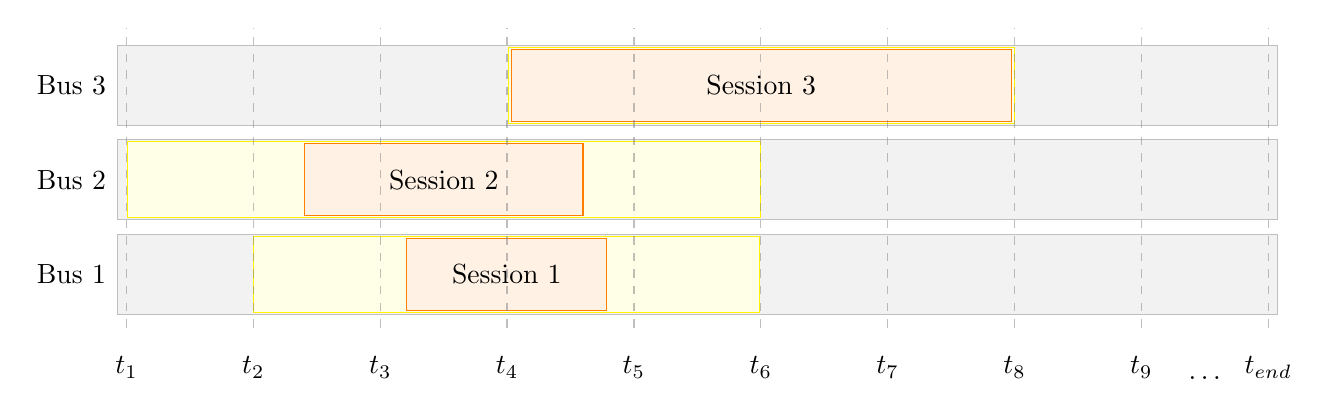
\begin{tikzpicture}
	\node[rectangle, draw=gray!50, fill=gray!10, minimum width=5.8in, minimum height=0.4in](bus1Box) at (7.75,0.8){};
	\node(bus1BoxLabel) at (-0.2, 0.8){Bus 1}; 
	\node[rectangle, draw=yellow!100, fill=yellow!10, minimum width=2.53in, minimum height=0.38in](charge11) at (5.33, 0.8){};
	\node[rectangle, draw=orange!100, fill=orange!10, minimum width=1in, minimum height=0.36in](charge111) at (5.33, 0.8){Session 1};

	\node[rectangle, draw=gray!50, fill=gray!10, minimum width=5.8in, minimum height=0.4in](bus2Box) at (7.75,2){};
	\node(bus1BoxLabel) at (-0.2, 2.0){Bus 2};
	\node[rectangle, draw=yellow!100, fill=yellow!10, minimum width=3.1625in, minimum height=0.38in](charge11) at (4.53, 2){};
	\node[rectangle, draw=orange!100, fill=orange!10, minimum width=1.3915in, minimum height=0.36in](charge111) at (4.53, 2){Session 2};
	
	\node[rectangle, draw=gray!50, fill=gray!10, minimum width=5.8in, minimum height=0.4in](bus3Box) at (7.75,3.2){};
	\node(bus1BoxLabel) at (-0.2, 3.2){Bus 3}; 
	\node[rectangle, draw=yellow!100, fill=yellow!10, minimum width=2.53in, minimum height=0.38in](charge11) at (8.56, 3.2){};
	\node[rectangle, draw=orange!100, fill=orange!10, minimum width=2.50in, minimum height=0.36in](charge111) at (8.56, 3.2){Session 3};


	\foreach \curLab/\preLab[count=\c, evaluate=\c as \pos using {0.5 + (\c - 1)*14.5/9}] in {t_1/t_1, t_2/t_1, t_3/t_2, t_4/t_3, t_5/t_4, t_6/t_7, t_7/t_6, t_8/t_7, t_9/t_8, t_{end}/t_9}
		{
			\node[label=below:$\curLab$](b\c) at (\pos, 0){};
			\node(t) at (\pos, 3.8){};
			\draw[dashed, line width=0.5pt, black!50, opacity=0.5] (b\c.north) -- (t.north); 
		}
		\path (b9.south) -- node[midway, below=0.1in]{$\hdots$}(b10.south); 
\end{tikzpicture}}
\caption{Demonstrates how results from $p_4$ can be reexpressed in terms of continuous variables} 
\label{fig:refactorExample}
\end{figure*}



\begin{figure*}
\centering
\scalebox{0.8}{
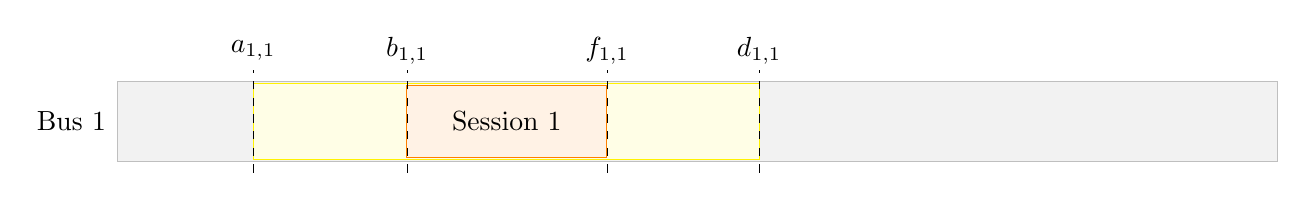
\begin{tikzpicture}
	\node[rectangle, draw=gray!50, fill=gray!10, minimum width=5.8in, minimum height=0.4in](bus1Box) at (7.75,0.8){};
	\node(bus1BoxLabel) at (-0.2, 0.8){Bus 1}; 
	\node[rectangle, draw=yellow!100, fill=yellow!10, minimum width=2.53in, minimum height=0.38in](charge11) at (5.33, 0.8){};
	\node[rectangle, draw=orange!100, fill=orange!10, minimum width=1in, minimum height=0.36in](charge111) at (5.33, 0.8){Session 1}; 
	\draw[dashed] (0.83in,0.15) -- (0.83in,1.45);
	\node at (0.83in,1.7){$a_{1,1}$};
	\draw[dashed] (3.36in, 0.15) -- (3.36in, 1.45);
	\node at (3.36in,1.7){$d_{1,1}$};
	\draw[dashed] (1.6in, 0.15) -- (1.6in, 1.45);
	\node at (1.6in,1.7){$b_{1,1}$};
	\draw[dashed] (2.6in, 0.15) -- (2.6in, 1.45);
	\node at (2.6in,1.7){$f_{1,1}$};
\end{tikzpicture}}
\caption{Gives variables of optimization for $p_5$}
\label{fig:secondProgramVars}
\end{figure*} 


\section{Charge Schedules}
The results from the Quadratic Program defined in the previous section give us a general estimate of how much and when buses should charge, however we must still address two primary issues. The first is defining concrete continuous time start and stop times for each charge sessionand the second is limiting the charge sessions to a finite number of chargers. After solving the first program, we take the results and derive {\it preliminary} intervals and average power consumptions for each charge session.  For example, consider a solution to a three bus, two charger scenario given in Fig. \ref{fig:solutionExample}.
Note that there appears to be three buses charging at the same time from $t_5$ to $t_6$ even though there are only two chargers.  We can reformulate this solution in terms of continuous start and stop variables and a variable charge rate so that the {\it duration} of each charge session may be relaxed. The objective is to store the given energy in the corresponding bus within the given charge interval.  Note how few of the charge sessions utilize the chargers to full capacity. This implies that there exists a smaller charge window in which equivalent power can be delivered. This allow us to use the charge durations from the solution from Fig. \ref{fig:solutionExample} as bounds on {\it allowable} charge windows instead of absolute truth. An example of how Fig. \ref{fig:solutionExample} may be reformulated is given in Fig. \ref{fig:refactorExample}. Note how the actual charge sessions don't necessarily need to take up all the time they were initially allocated in the first solution and that these times can fluctuate if the average charge rate is less than the maximum charger capacity. In this example, we assume a maximum charge capacity of 350kW.  Note how the third charge session does have to be exactly where it was scheduled because the average is equal to the maximum charge rate.
If we examin just the schedule for Bus 1, we note that there are four essential variables for the corresponding charge session: $a(i,r)$, $b(i,r)$, $f(i,r)$ and $d(i,r)$ which represent the minimum start time, actual start time, actual end time, and maximum end time respectively. The problem we must now solve is one of arranging these ``rectangles'' such that each one is larger than it's minimum width (or charge time).  We must also account for the number of chargers. It can be helpful to view the problem as a bin packing problem, where each session must fit within the ``swim lane'' of a charger.  For example, taking the charge sessions given in Fig. \ref{fig:refactorExample} and arranging them so that there is no overlap between sessions will yield a valid solution as shown in Fig. \ref{fig:secondSolutionExample}.
\par From Fig. \ref{fig:secondProgramVars}, we know that $a(i,r), b(i,r),f(i,r)$ and $d(i,r)$ must be such that 
\begin{equation*}\begin{aligned}
	a(i,r) \le b(i,r) \\
	b(i,r) \le f(i,r) \\
	f(i,r) \le d(i,r). 	
\end{aligned}\end{equation*}
Where $a(i,r)$ and $d(i,r)$ are known from the previous optimization problem, and $b(i,r)$ and $f(i,r)$ are optimization variables.
\par We desire to solve this second optimization method in a greedy fashion using a heuristic approach. Let $\mathcal{B}$ be the set of all charge sessions which are sorted according to their {\it latest} start time.  Begin by removing the first, or earliest, $n_{\text{charger}}$ sessions and placing them in separate queues for a charger. For the remainder of the charge sessions, we remove the next item from the list, determine which chargers are available to service this request by checking that the previous service can finish before the next will start, and then select the charger which yields the smallest amount of overlap in session availability.
\begin{algorithm}[!ht]
\DontPrintSemicolon
\KwIn{Sorted List of Charge Sessions}
\KwOut{Charge Schedule for Each Charger}
\For{i = 1:$n_{\text{charger}}$}
{
	charger[i].append(inputList.pop())
}
\While{inputList not empty}
{
	item = inputList.pop()\;
	\For{i = 1:$n_{\text{charger}}$}
	{
		bestOverlap = inf\;
		bestCharger = -1\;
		\If{charger $i$ is available}		
		{
			\If{overlap is less than bestOverlap}
			{
				bestOverlap = itemOverlap\;
				bestCharger = i\;
			}
		}
	}
	charger[bestCharger].append(item)\;
}
\caption{Pseudocode that illustrates how charge sessions are assigned}
\label{alg:chargeAssign}
\end{algorithm}

%\input{8_results.tex}
%\input{9_future.tex}
\section*{Acknowledgment}This material is based in part upon work supported by the National Science Foundation through the ASPIRE Engineering Research Center under Grant No. EEC-1941524, the Department of Energy through a prime award with ABB under Grant No. DE-EE0009194, and PacifiCorp under contract number 3590. Any opinions, findings, and conclusions or recommendations expressed in this material are those of the authors and do not necessarily reflect the views of the National Science Foundation, the Department of Energy, or Pacificorp.
%\newpage 
\onecolumn	
\newcommand{\coloredhline}{\arrayrulecolor{gray!20} \hline \\[0.01in]\arrayrulecolor{black}}
\newcommand{\myendline}{\\ \coloredhline}
\label{tab:paperVariables}
\centering
\begin{supertabular}{b{0.06\textwidth} m{0.3\textwidth} m{0.09\textwidth} m{0.06\textwidth} m{0.3\textwidth} m{0.09\textwidth}}
	\toprule%----------------------------------------------------------------------------
	\textbf{Variable} & \textbf{Description} & \textbf{Range} & \textbf{Variable} & \textbf{Description} & \textbf{Range}\\
	\toprule%-----------------------------------------------------------------------------
	\multicolumn{6}{l}{Indices} \myendline
	i & Bus index     & $\mathbb{N}$ & j & Time Index & $\mathbb{N}$\\ \myendline
	k & Charger index & $\mathbb{N}$ & r & Route Index \\[0.15in]
	\hline \\[-5pt]
	\multicolumn{6}{l}{Formulation} \\[-9pt]\myendline
	$n_{\text{bus}}$&\parbox{0.3\textwidth}{The number of buses in the optimization framework.}                                                           & $\mathbb{Z}$            & $n_{\text{time}}$                      &\parbox{0.3\textwidth}{ The number of time indices in a day.                                                                                 }      & $\mathbb{Z}^+$ \\\myendline
	$b_{p(i,j)}$   & \parbox{0.3\textwidth}{The average power consumed by bus $i$ during time period $j$.}                                                                              & $\mathbb{R}$           & $t_j$         &\parbox{0.3\textwidth}{ The time at time index $j$. This paper also refers to the period of time from $t_j$ to $t_{j+1}$ as ``period $t_j$''.}      & $\mathbb{R}$\\\myendline 
	$\bm{b}$       & \parbox{0.3\textwidth}{A vector containing each value for $b_{p(i,j)}$.}                                                                                          & $\mathbb{R}^{n_{\text{bus}}\cdot n_{\text{time}}}$           & $\alpha(i,j)$ &\parbox{0.3\textwidth}{the percentage of time bus $i$ spends in the station from $t_j$ to $t_{j+1}$. }                              & $[0,1]$\\\myendline
	$\mathcal{A}$  & \parbox{0.3\textwidth}{The set of all $i\times j$ elements where bus $i$ can charge at time index $j$}                                  & $i\times j$             & $p_{\text{max}}$ &\parbox{0.3\textwidth}{The maximum power a bus charger can deliver to a bus in kW. This paper assumes a value of 350 for most examples and results.} & $\mathbb{R}^+  $\\\myendline
	$\mathcal{\tilde{A}}$  & \parbox{0.3\textwidth}{The complement of $\mathcal{A}$.}                                                                        & $i\times j$  \\[0.5in]
	\hline \\[-0.07in]
	\multicolumn{6}{l}{Battery} \\[-9pt] \myendline
	$h_{\text{min}}$ & The minimum allowable state of charge                           & $\left ( 0,h_{\text{max}} \right )$                & $h_{\text{max}}$  & The maximum state of charge                                                   & $\mathbb{R}^+$                                     \\ \myendline 
	$\eta_i$         & The beginning state of charge for bus $i$                       & $\left ( h_{\text{min}}, h_{\text{max}} \right )$  & $h(ij)$           & The state of charge for bus $i$ at time $t_j$. & $\left ( h_{\text{min}}, h_{\text{max}} \right )$\\ \myendline
	$\Delta T$       & The change in time from $t_j$ to $t_{j+1}$                      &$\mathbb{R}^+ $  & $\bm{h}$             & A vector containing all state of charge values.                                        & $\mathbb{R}_+^{n_{\text{bus}}\cdot n_{\text{time}}}$                                   \\ \myendline
	$\delta(ij)$     & The battery discharge for bus $i$ during time period $j$.               & $\mathbb{R}_+$                                     & $h(i,\text{end})$& Bus $i$'s final state of charge.                                              & $\left ( h_{\text{min}}, h_{\text{max}} \right )$\\[0.3in]
	\hline \\[-0.07in]
	\multicolumn{6}{l}{Charger Management} \\[-9pt] \myendline 
	$n_{\text{charger}}$             & The time index for the start of bus $i$'s $j^{\text{th}}$ stop                                                    & $\mathbb{Z}_+$                   & $p_c(j)$            & The average power consumed by all buses during time period $j$. & $\mathbb{R}$                    \\ \myendline
	$\bm{p_c}$                       & A vector containing all values of $p_c(j)$.                                                                       & $\mathbb{R}_{+}^{n_{\text{time}}}$                   & $J_{\text{thrash}}$          & A secondary objective function which penalizes multiple plug-in instances per charge session.& $\mathbb{R}_+$                  \\[0.3in] 
	\hline \\[-0.07in]
	\multicolumn{6}{l}{Objective}  \\[-9pt] \myendline
	$\mu_{\text{e-on}}$         & On-Peak Energy Rate                                                            & $\mathbb{R}_+$                                & $\mu_{\text{e-off}}$       & Off-Peak Energy Rate                                                                                     & $\mathbb{R}_+$                 \\ \myendline
	$\mu_{\text{p-on}}$         & On-Peak Demand Power Rate                                                      & $\mathbb{R}_+$                                & $\mu_{\text{p-all}}$       & Facilities Power Rate                                                                                    & $\mathbb{R}_+$                 \\ \myendline
	$\mathcal{S}_{\text{on}}$   & The set of on-peak time indices                                                & \scalebox{0.9}{$\{1,...,n_{\text{time}}\}$}   & $p_{\text{demand}}$        & Maximum average power during on-peak periods                                                             & $\mathbb{R}$                 \\ \myendline
	$p_{\text{facilities}}$     & Maximum average power over all time instances.                                 & $\mathbb{R}_+$                                & $p_t(j)$                   & The total average power co nsumed by both the bus chargers and the uncontrolled loads.                    & $\mathbb{R}_+^{n_{\text{time}}}$  \\ \myendline
	$u(j)$                      & The average power over time $j$ consumed by the uncontrolled loads             & $\mathbb{R}_+^{n_{\text{time}}}$            & $\bm{p}_t$                 & a vector containing $p_t(i)$ for all $i$.                                                                  & $\mathbb{R}_+^{n_{\text{time}}}$ \\ \myendline 
	$e_{\text{on}}$             & The total amount of energy consumed by the bus chargers and uncontrolled loads during off-peak hours.& $\mathbb{R}_+$                              & $e_{\text{off}}$             & The total energy consumed by the bus chargers and uncontrolled loads during on-peak hours.               & $\mathbb{R}_+$ \\ \myendline 
	$J_{\text{cost}}$           & The section of the objective function pertaining to the fiscal expense of charging buses. & $\mathbb{R}$                & $J_{\text{all}}$               & The expression for the complete objective function. & $\mathbb{R}$ \\[0.3in]
	\hline \\[-0.07in]
	\multicolumn{6}{l}{Charge Schedules}  \\[-9pt] \myendline
	$a(i,r)$ & The beginning of the allowable charge interval for bus $i$'s $r^{\text{th}}$ charge session. & $\mathbb{R}_+$ & $b(i,r)$ & The commanded start time for bus $i$'s $r^{\text{th}}$ charge session& $\mathbb{N}$\\ \myendline
	$f(i,r)$ & The commanded end time for bus $i$'s $r^{\text{th}}$ charge session. & $\mathbb{R}_+$ & $d(i,r)$ & The end time of the allowable charge interval for bus $i$'s $r^{\text{th}}$ charge session. & $\mathbb{R}_+$ \\\myendline
	%
\end{supertabular}
\twocolumn

\printbibliography
\end{document}


